Una trasformazione morfologica è una semplice operazione  basata sulla shape (high x width) dell’immagine.


\begin{minted}
[
  xleftmargin=\parindent,
  framesep=2mm,
  baselinestretch=1.2,  
  fontsize=\footnotesize,
  linenos
]
{python}

kernel = cv2.getStructuringElement(cv2.MORPH_ELLIPSE, (5, 5))
blackhat = cv2.morphologyEx(cimg, cv2.MORPH_BLACKHAT, kernel)
bottom_hat_filtered = cv2.add(blackhat, cimg)    
\end{minted}

Nel codice sopra riportato la funzione che opera le trasformazioni morfologiche è \texttt{cv2.morphologyEx}, la quale utilizza erosione e dilatazione come operazioni di base. L’erosione consiste nell’erodere i bordi di una forma, un pixel nell’immagine originale in bianco e nero (0 o 1) sarà considerato 1 solo se tutti i pixels coperti dal kernel sono 1, altrimenti è eroso (messo a zero). La dilatazione invece effettua il processo inverso dell’erosione. MorphologyEx necessita di due input, il primo è l’immagine originale, il secondo è chiamato structuring element o kernel. Specificando come parametro della funzione \texttt{cv2.getStructuringElement MORPH\_ELLIPSE} si ricava un elemento strutturale a forma di ellisse inscritta in un rettangolo, tale elemento viene poi utilizzato come kernel effettivo per ricavare il blackhat. Questo tipo di operazione mette in risalto regioni scure dell’immagine con uno sfondo luminoso. Il passo finale è l’applicazione del blackhat all’immagine in grayscale, il risultato è chiamato bottom hat.


\begin{figure}[h]
  \centering
  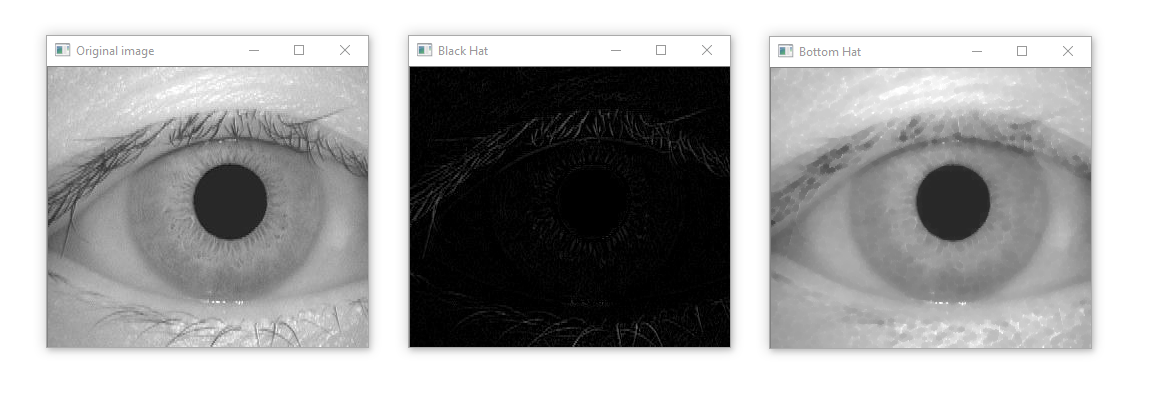
\includegraphics[width=1.0\textwidth]{black_hat}
  \caption{Applicazione della trasformazione black hat all'immagine}
\end{figure}

La scelta di queste trasformazioni morfologiche risiede nel fatto che si adattano molto bene alla successiva applicazione di un blur, in particolar modo del Gaussian Blur.
